\chapter{Asking Strangers How Much MONEY They Make (Austin, Texas)}

We begin with a question that is at once numerical and social: what was the most amount of money someone ever made in a single year? The lecture does not answer that question cleanly; it uses the discomfort around it to open a wider discussion of finance, management, networking, risk, assets, and long-horizon planning. There is no literal board mathematics in this interview, but there is a clear mathematical spine: a sequence of contrasts, orderings, and update rules that we can write down schematically without pretending that the street interview turned into a formal theorem.

\begin{remark}
The formulas below are companion-note reconstructions of the lecture's logic. They preserve explicit comparisons and transitions from the transcript, while remaining modest about what was actually stated and what is only being organized.
\end{remark}

\section{Opening Pressure and the Interview Device}

The lecture opens by pressing the most volatile question first. Before we know the speakers well, before we know the industries, before we know the advice, we are asked to sit in the discomfort of money disclosure. One person refuses, another dodges, another discloses only partially. Even the early snippets --- a software executive declining to disclose, an entrepreneur saying ``we spend money, we make money'' --- belong to the same opening maneuver. They tell us that wealth talk is never just arithmetic; it is also posture, privacy, and selective revelation.

\begin{equation}
Q_{\mathrm{income}} \longrightarrow \{\text{refusal},\ \text{evasion},\ \text{partial disclosure},\ \text{boast}\}.
\end{equation}

Only then does the host widen the frame. We are told that the team is moving around downtown Austin and asking strangers about the most money they have made in a single year. The channel's own history is introduced in passing, with the claim that it reached roughly \(1.4\) million followers. That number should remain in the notes, not because it changes the theory, but because it tells us how the host wants the encounter to be read: not as a one-off conversation, but as part of a repeated method.

What follows therefore has a double rhythm. Each interview is local and personal, but the host's repeated question keeps turning those local answers into comparable cases.

\section{The First Substantive Case: Finance Before Vision}

The first extended case begins with industry identification. The guest places himself in neurotechnology and describes his work, in his own terms, as using frequencies and digital frequency patterns to restore health and to help get people off psychiatric medication. We should preserve that description as the speaker's own claim and then follow the lecture where it actually goes next: not into technical neuroscience, but into entrepreneurial hindsight.

The real question is what one would say to one's younger self at the start of a first business. The answer is immediate and bracingly practical: be careful financially. The lecture does not start with dream, scale, or mission. It starts with the cost of financing errors.

\begin{equation}
B_{\mathrm{bank}} \prec \{S_{\mathrm{self}},\,F_{\mathrm{friends/family}},\,P_{\mathrm{platforms}}\}.
\end{equation}

Here \(B_{\mathrm{bank}}\) denotes bank borrowing, \(S_{\mathrm{self}}\) self-funding, \(F_{\mathrm{friends/family}}\) relationship capital, and \(P_{\mathrm{platforms}}\) platform-based raising. The notation is schematic, but the order is faithful to the transcript. The speaker says plainly that the biggest mistake he ever made was letting banks lend him money. That does not prove a universal capital theorem; it does establish a strong preference ordering inside the lecture.

We can make the speaker's practical reasoning more explicit:
\begin{enumerate}
\item The business begins with uncertainty.
\item Borrowed bank money adds external pressure before the business has stabilized.
\item That pressure constrains later freedom of movement.
\item Therefore, when possible, we prefer funding sources that preserve flexibility.
\end{enumerate}

This is the first real mathematical move in the chapter. We are not computing interest schedules. We are ordering financing mechanisms by how much strategic regret they are likely to create.

\section{Scaling: From Vertical Command to Horizontal Work}

Once the lecture has fixed attention on financing, it pivots to a second question: how does one scale a business? Again the answer does not arrive as a KPI or spreadsheet heuristic. It arrives as a contrast in shape.

\begin{definition}
Let \(M_v\) denote vertical management and \(M_h\) denote horizontal management. In the lecture's own language, \(M_v\) places managers above the group, where they ``bark'' and issue orders downward, while \(M_h\) places the working participants laterally, at the same level, where they sit together and work together.
\end{definition}

\begin{align}
M_v &: \text{orders flow downward},\\
M_h &: \text{work proceeds laterally},\\
M_h + C &\Rightarrow D_{\mathrm{final}}.
\end{align}

Here \(C\) is a critical moment and \(D_{\mathrm{final}}\) is the final decision taken by rank. This is the refinement that gives the lecture its real structure: horizontal management does not abolish leadership. It merely refuses to make hierarchy the default state of every decision.

\begin{figure}[h]
\centering

\includegraphics[width=0.72\textwidth]{lecture_113_figure_02.png}
\caption{The speaker's gesture gives the lecture's key visual evidence for horizontal management: both hands are spread at the same level while he describes managers who work together across the table.}
\end{figure}

The screenshot matters because it is the chapter's one direct visual diagram, even though nothing is literally drawn. The hands are level, lateral, and non-stacked. The subtitle is slightly garbled, but the geometry is clear. What the lecture says verbally --- ``horizontal managers'' --- is what the gesture says visually.

\begin{figure}[h]
\centering
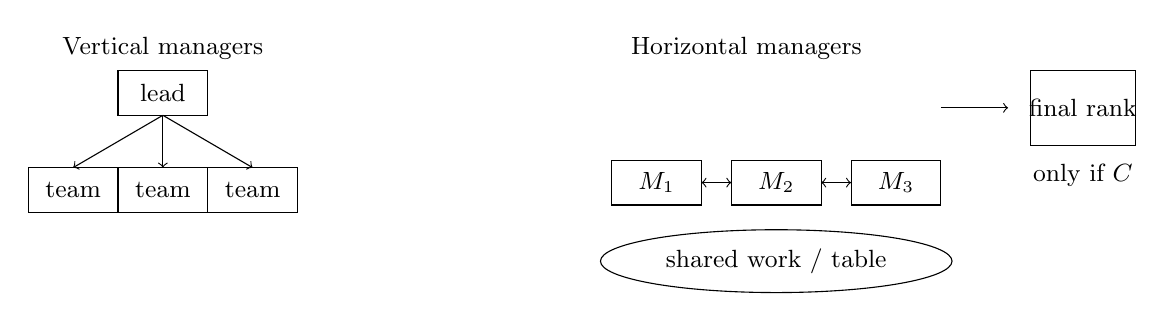
\begin{tikzpicture}[scale=0.95]
\node at (-4.3,3.1) {\small Vertical managers};
\draw (-4.9,2.2) rectangle (-3.7,2.8);
\node at (-4.3,2.5) {\small lead};
\draw (-6.1,0.9) rectangle (-4.9,1.5);
\draw (-4.9,0.9) rectangle (-3.7,1.5);
\draw (-3.7,0.9) rectangle (-2.5,1.5);
\node at (-5.5,1.2) {\small team};
\node at (-4.3,1.2) {\small team};
\node at (-3.1,1.2) {\small team};
\draw[->] (-4.3,2.2) -- (-5.5,1.5);
\draw[->] (-4.3,2.2) -- (-4.3,1.5);
\draw[->] (-4.3,2.2) -- (-3.1,1.5);

\node at (3.5,3.1) {\small Horizontal managers};
\draw (1.7,1.0) rectangle (2.9,1.6);
\draw (3.3,1.0) rectangle (4.5,1.6);
\draw (4.9,1.0) rectangle (6.1,1.6);
\node at (2.3,1.3) {\small \(M_1\)};
\node at (3.9,1.3) {\small \(M_2\)};
\node at (5.5,1.3) {\small \(M_3\)};
\draw[<->] (2.9,1.3) -- (3.3,1.3);
\draw[<->] (4.5,1.3) -- (4.9,1.3);
\draw (3.9,0.25) ellipse (2.35 and 0.42);
\node at (3.9,0.25) {\small shared work / table};

\draw[->] (6.1,2.3) -- (7.0,2.3);
\draw (7.3,1.8) rectangle (8.7,2.8);
\node at (8.0,2.3) {\small final rank};
\node at (8.0,1.4) {\small only if \(C\)};
\end{tikzpicture}
\caption{A cautious reconstruction of the lecture's management contrast. The right-hand diagram is transcript-backed and frame-supported; the left-hand contrast is transcript-backed but not directly visible in the frame.}
\end{figure}

\subsection{Question \& Answer}

\paragraph{Question.} How do we scale a business without collapsing into pure command-and-control?

\paragraph{Answer.} The lecture's answer is to reverse the default order. We do not begin with rank and then ask collaboration to survive underneath it. We begin with shared work, shared table, and shared listening. Only when a critical moment arrives do we pull rank and make a final decision.

A minimal update rule is therefore
\begin{align}
\neg C_t &\Rightarrow \text{remain in } M_h,\\
C_t &\Rightarrow D_{\mathrm{final}}.
\end{align}

The speaker then broadens the point. Scaling is not merely a structural chart; it is a choice about the kind of people we gather. We surround ourselves with professionals, aspiring professionals, or like-minded people in the vision. Then comes the moral clause that keeps the whole section from becoming managerial jargon: we listen. The lecture says explicitly that people are now ready for the fight, ready for the corner, ready to go after it. That posture, we are told, should not be imported into the business.

\section{Reset, Breadth, and the Logic of Network}

At this point the lecture does something important for pacing. It pulls back from the first substantial interview and briefly explains the Hard Knocks method itself. The host remarks that interviews happen everywhere: at the ice-cream shop, at the convenience store, while waiting in line, whenever someone looks like they might have something to say. This is not filler. It re-motivates the format before the next conceptual cluster begins.

The next executive case starts in software marketing and with a question about entering tech. The answer is not specialization at the outset, but breadth. The speaker describes moving through multiple startups, touching different parts of the business, and learning faster than he would have if he had locked himself too early into a comfortable high-paying role. This is a real progression in the lecture:
\begin{align}
\text{exposure} &\longrightarrow \text{breadth of tasks},\\
\text{breadth of tasks} &\longrightarrow \text{faster learning},\\
\text{faster learning} &\longrightarrow \text{later earning power}.
\end{align}

Only after that sequence does the lecture return to the annual-income question, and the answer remains deliberately imprecise: high six figures, really high six figures. The imprecision matters. The lecture is not trying to produce clean salary data; it is trying to make the reader feel how selective disclosure and commercial self-description interact.

Now the lecture reaches one of its most explicit conceptual oppositions.

\subsection{Question \& Answer}

\paragraph{Question.} Which matters more, who you know or what you know?

\paragraph{Answer.} The lecture lets the blunt answer come first: who you know matters. But it then corrects the naïve reading of that slogan. Network opens the door; value determines whether the relationship survives.

\begin{equation}
A_{\mathrm{network}} \xrightarrow{\,V_{\mathrm{provided}}\,} R_{\mathrm{continued}}.
\end{equation}

Here \(A_{\mathrm{network}}\) is access through a network, \(V_{\mathrm{provided}}\) is value brought into the relationship, and \(R_{\mathrm{continued}}\) is continued access or durable connection. The lecture presses this hard: if one has nothing to bring to the table, the chain does not propagate.

\begin{equation}
V_{\mathrm{provided}} = 0 \Rightarrow R_{\mathrm{continued}} \to 0.
\end{equation}

This is only a schematic rendering, but it captures the exact logical correction the lecture makes. We may enter high-value circles through introductions, but we do not remain there by introduction alone.

The same interview adds the related claim that ``you are a brand.'' That line should not be treated as motivational fluff. In the lecture it serves as a further tightening of the same rule. We do not know whom we are going to meet, so ordinary social conduct is already part of professional positioning. Social life leaks into commercial life; the membrane between them is thin.

\section{Risk, Competition, and the Ethics of Commercial Conduct}

The lecture then hardens. A medical-business owner refuses the exact income question, answers ``a lot'' when pressed, and from there turns toward a more severe doctrine of work. Working for oneself, he says, is not for everybody. He describes a stem cell company that has been running for seventeen years and doing more than \$4 million in revenue. The quantitative claims matter, but they matter mainly because they anchor the tone of what follows.

The sequence is important. First, one must take chances. Second, after the first hiring threshold, school prestige matters much less than many young people suppose. Third, once we are out in the market, we are not in a protected environment. We are in competition against people who have been doing this for decades.

This section could easily become mere aggression, but the lecture refuses to leave it there. The speaker recalls his father's advice: people buy from people they like. That sentence turns the section back toward the earlier networking beat. Commercial life is personal before it is technical. The second paternal rule --- do not sweat the small stuff; control the controllables --- then completes the correction. Risk is not frenzy. Competition is not panic. The lecture is trying to teach composure inside exposure.

We may summarize this section by a simple pair of rules:
\begin{align}
\text{risk without movement} &\Rightarrow \text{stagnation},\\
\text{risk without composure} &\Rightarrow \text{noise}.
\end{align}

The lecture wants neither passivity nor noise. It wants active, controlled commercial conduct.

\section{Assets, Liquidity, Creation, and Planning Backward}

The late lecture pivots from posture and network to portfolio mechanics. A former military interviewee explains that, at each duty station, he bought a house; when he moved, he kept the prior one and rented it out. In this manner, almost before the speaker explicitly named the pattern, a side practice became an investment portfolio.

\begin{equation}
P_{\mathrm{base\ houses}} \to P_{\mathrm{rentals}} \to (\text{asset rich},\,\text{cash poor}) \to L_{\mathrm{liquid}}.
\end{equation}

That line captures the logic cleanly. Repeated purchases become rentals; rentals become accumulated assets; accumulated assets produce a balance-sheet state in which wealth is present but cash is tight; and that state motivates liquidation when the investor wants optionality for the next move. The guest's reported annual range --- between \$500{,}000 and \$600{,}000 --- matters less than this structural sequence.

The next entrepreneur then shifts the lecture from asset accumulation to active design. If one wants to be a millionaire, he says, one should create. One should create something new, or fix what is broken, or recreate something already working and add one's own spin, knowledge, and format to it.

\begin{align}
X_{\mathrm{existing}} &\xrightarrow{\text{own spin + knowledge}} X'_{\mathrm{recreated}},\\
T_{\mathrm{target}} &\to \{c_i\}_{i=1}^{n} \to s_1.
\end{align}

The first line records the recreation rule. The second records the backward-planning rule. The lecture does not merely tell us to have a plan; it gives a procedural example of what planning means.

\paragraph{Worked example.} The pool-building example is the clearest place where the lecture unfolds step by step.
\begin{enumerate}
\item Fix the target operation: a business that builds pools.
\item Decompose that target into required trades and execution layers: mechanical work, electrical work, plumbing, gunite, shotcrete, concrete, and the rest.
\item Identify who performs each part, where they are found, and how reliable they are.
\item Only then choose the first move.
\end{enumerate}

The direction of reasoning is the point. We do not drift forward from vague desire; we work backward from a specified endpoint. This same guest also gives the lecture one of its more useful volatility facts: annual income may be about \$650{,}000, while month to month it can swing from \$75{,}000 to \$10{,}000. The notes should preserve that because it teaches the reader not to confuse a good year with a smooth year.

\section{Two Buckets and the Portability of Skill}

The closing movement widens the lecture beyond entrepreneurship narrowly understood. An LAPD veteran says that, through celebrity weddings and security work, he once topped \$300{,}000. Yet the more durable lesson is not about side-income glamour. It is about financial structure. His training officer told him not to depend on pension alone, but to build a second bucket through deferred compensation.

\begin{equation}
W_{\mathrm{retirement}} = W_{\mathrm{pension}} + W_{\mathrm{deferred\ comp}}.
\end{equation}

This should remain simple. The lecture is not deriving a retirement model. It is emphasizing diversification across time. Two buckets are better than one bucket if one wants future optionality.

The last interview cools the tone even further. A cybersecurity and privacy professional says that the best decision of his life was to major in engineering. The reason is not that everyone must remain an engineer, but that engineering teaches problem solving, and problem solving travels.

\begin{equation}
\text{engineering training} \longrightarrow \text{problem solving} \longrightarrow \text{career optionality}.
\end{equation}

This is the right closing note. The lecture began with the discomfort of income disclosure and ends with a calmer, more structural thought: the best long-horizon decisions are often the ones that preserve our ability to move across domains without losing usefulness.

\section{Summary}

The lecture opens with a social provocation and then steadily converts it into a sequence of commercial rules. First, financing matters, and the wrong debt can become a lasting regret. Second, scaling is not merely about authority; it is about when authority should and should not appear. Third, network matters, but only value makes network durable. Fourth, risk must be paired with composure, likability, and control of the controllables. Fifth, assets, liquidity, and creation belong to different stages of wealth-building and should not be confused. Finally, long-horizon financial stability and career freedom come from structure: multiple buckets, portable training, and the ability to solve problems in more than one setting.

That is the chapter's real mathematics. We are not computing from a board. We are formalizing a sequence of choices, relations, and transitions that the lecture keeps returning to, each time from a different human angle.